\section[Introduction]{Introduction}
\epigraph{\centering \textit{“Things like chatbots, machine learning tools, natural language processing, or sentiment analysis are applications of artificial intelligence that may one day profoundly change how we think about and transact in travel and local experiences.”}}{Gillian Tans}

Sentiment Analysis or Opinion Mining is a way of finding out the polarity or strength of the opinion (positive or negative) that is expressed in written text.
is used in business to understand social sentiment for their brand, a particular product or service.

\subsection[In the previous episodes]{In the previous episodes}
In the last semester, my project partner and I have for the first time stepped into the world of sentiment analysis, making use of various supports such as tutorials, explanations, and lots of research.
We then decided to use all the material we had found to build something of our own, so we tried to do a project categorizing the sentiment of hotel reviews.
We wanted to split the sentiment of the reviews into 5 categories: from awful to excellent.
At the end of the project, we managed to have an accuracy of about 0.48, taking into consideration the 5 categories was a very good result.


\subsection[Project description]{Project description}
\label{main}
The thesis project I am working on this semester, will still be on sentiment analysis, this time the model created will be used to make predictions about newspaper news, to understand the polarity of an article or the newspaper itself.
With the current rapid developments in Deep Learning, many new technologies for text analysis have emerged.
This project will make use of these technologies and develop its own "Sentiment Analysis Model".
This model can basically be imagined as a function that takes arbitrary text as input, evaluates it and classifies it into a scale of emotions from negative to positive.
To develop and train a model with this capability requires many prebuilt datasets of real examples from the Internet. These are then used to feed the model so that it can learn from these datasets and deduce correlations. Based on these correlations, the model will then be able to process arbitrary texts and assign sentiment values to them.


\subsection{Motivation}
As already mentioned, this technology allows you to crystallize negative and positive feelings from a text. Besides sentiment classification, sentiment analysis brings many other benefits in areas such as marketing and customer satisfaction. Some of these benefits could be, for example:

\begin{itemize}
\item \textbf{Customer classification}\\
Sentiment analysis allows customers to be classified according to their emotional mood. This offers the opportunity to find customers who are more willing to buy.
\item \textbf{Chatbot training}\\
With the results of the Sentiment Analysis Tool, it is possible to train chatbots to recognize and respond to specific customer sentiments.
\item \textbf{Scalability and automation}\\
As a digital tool, Sentiment Analysis can be easily extended or integrated into an automated system.
\end{itemize}

From these points, a strongly increasing tendency regarding the application of sentiment analysis can be assumed. This makes it all the more relevant for developers to get to grips with it. From the developer's perspective, learning sentiment analysis also promotes new experiences in areas such as: 

\begin{itemize}
\item Data analytics
\item Data science
\item Machine learning
\item Predictive modelling
\end{itemize}

\subsection[Goal]{Goal}
\label{main}
The core of this project is with the help of different tools like Tensorflow\cite{tensorflow}, Keras and BERT to create a "model" that takes text as input and classifies it in “positive” or “negative”. 
To calculate the polarity of the article, I will use different datasets so that I can train and test the model and see if with different datasets there different results are.
Unfortunately, due to an impediment, my partner from the previous project was not able to take part in this assignment, which means that I must continue this project alone.
For a matter of timing and difficulty, I have resized the project and the categories on which to make a prediction will no more be 5 as in the last project, but 2.
This model should be available as a single component that can be integrated into arbitrary applications.\\
For the implementation of the project, I have used several websites and tutorials:
\begin{itemize}
    \item Tutorial for Keras\cite{tutorial_keras}
    \item Deep-Learning-For-Hackers\cite{git}
    \item Sentiment Analysis with TensorFlow 2 and Keras\cite{tutorial}
    \item Deep Learning LSTM for Sentiment Analysis\cite{karikari_deep_2020}
    \item Natural Language Processing and Sentiment Analysis using Tensorflow.\cite{khan_natural_2020}
    \item Sentiment Analysis: First Steps With Python's NLTK Library \cite{python_sentiment_nodate}
    \item Sentiment Analysis using Deep Learning with Tensorflow \cite{pandey_sentiment_2020}
    \item Practical Text Classification With Python and Keras \cite{python_practical_nodate}
    \item Classify text with BERT \cite{noauthor_classify_nodate}
    \item Text Classification with BERT using Transformers for long text inputs \cite{girdhar_text_2020}
    \item Simple Transformers — Multi-Class Text Classification with BERT, RoBERTa, XLNet, XLM, and DistilBERT \cite{rajapakse_simple_2019}
    \item Fine-tuning BERT with Keras and tf.Module \cite{antyukhov_fine-tuning_2020}
\end{itemize}

\subsection{Project organization}
The table~\ref{tab:Organisation} describes who occupies which role in our project organization:
\begin{longtable}[ c ]{| m{5cm} | m{5cm}|  m{3cm}|}
 \hline
 \multicolumn{3}{| c |}{\textbf{Project organization}}\\
 \hline
 \textbf{Role in the \newline project organization} & \textbf{Name}  & \textbf{BFH\newline Abbreviation}\\
 \hline
 \endfirsthead
%
 \multicolumn{3}{c}%
 {{\bfseries Table \thetable\ continued from previous page}} \\
 \hline
 \textbf{Role in the \newline project organization} & \textbf{Name}  & \textbf{BFH Abbreviation}\\
 \hline
 \endhead
%
{Tutor}   & {Mascha Kurpicz-Briki}  & {kim3}   \\ \hline
{Expert}  & {Andreas Dürsteler}         & {-}   \\ \hline
{Developer}     & {Giorgio Bakhiet Derias}& {bakhg1}\\ \hline
                 
\caption{Project organization}
\label{tab:Organisation}\\
\end{longtable}

\subsection{Tools}
In the table~\ref{tab:Tools} you can find the different tools I used for this project:
\begin{longtable}[ c ]{| m{4cm} | m{10cm}|}
 \hline
 \multicolumn{2}{| c |}{\textbf{Tools}}\\
 \hline
 \textbf{Tool}  & \textbf{Description}\\
 \hline
 \endfirsthead
%
 \multicolumn{2}{c}%
 {{\bfseries Table \thetable\ continued from previous page}} \\
 \hline
\textbf{Tool}  & \textbf{Version}\\
 \hline
 \endhead
%
{\gls{jupyter}}           & {A document that can store code, diagrams, graphics and much more.}      \\ \hline
{Google   \gls{colab}oratory} & {Online platform to host \gls{jupyter}.} \\ \hline
{\gls{kaggle}}   & {Is an online machine learning environment and community.}      \\ \hline  
{\gls{anaconda}}          & {Application to manage libraries of larger projects.}      \\ \hline
{\gls{virtual machine}}   & {\gls{anaconda} is installed on the virtual machine to run the project.}      \\ \hline
{PyCharm}   & {IDE used for the Python language. It is developed by the company JetBrains.}      \\ \hline
{GitHub}   & {GitHub is a hosting service for software projects.}      \\ \hline
{Overleaf}   & {Overleaf is a cloud-based collaborative LaTeX editor used to write, edit, and publish scientific papers.}      \\ \hline
{MLMP}   & {MLMP is a cloud-based environment for machine learning created by BFH.}      \\ \hline
{\gls{Scikit-learn}}           & {Open source machine learning software library for the Python programming language.}      \\ \hline
{Tensorflow}   & {Open source software library for machine learning.}      \\ \hline
{\gls{keras}}             & {Tensorflow library specifically for creating neural networks.}      \\ \hline
{Ktrain}   & {is a library to help build, train, debug, and deploy neural networks in the deep learning software framework Keras.}      \\ \hline
{BERT}   & {Is a recent paper published by researchers at Google AI Language.}      \\ \hline
{Hugging Face}   & {Is an open-source provider of natural language processing (NLP) technologies.}      \\ \hline

 

\caption{Tools}
\label{tab:Tools}\\
\end{longtable}


\subsection{The development environment}
This section will explain all the components used for the development environment. 
\subsubsection{Jupyter Notebook}
The model is developed in the form of a \gls{jupyter} notebook using the Python programming language. \gls{jupyter} notebooks are documents that can contain code, text, images, diagrams and explanations. This is especially suitable for this project, because in Machine Learning it is often useful to explain the sourecode with graphs and diagrams.

\subsubsection{Google \gls{colab}oratory}
The notebook was initially hosted on Google \gls{colab}oratory\cite{colab}. This brought the following advantages:
\paragraph{Synchronization} 
By storing the notebook in a central location, Google Drive, and having everyone access the same notebook, all changes are immediately visible to all users of the notebook.
\paragraph{Project structure} 
The \gls{jupyter} allows to map the whole project in a structured way in a single file. 
\paragraph{Project dependencies}
Since the project is hosted on Google \gls{colab}, it is not necessary as a developer to install libraries and other dependencies locally.

However, as it turned out, \gls{colab} removes from the platform external resources that were imported into the project after a certain time. This meant that I had to re-import the datasets, which are essential for the development of my model, before each work. This forced me to set up a \gls{virtual machine} on which the notebook can then be run locally.

\subsubsection{The \gls{virtual machine}}
In order to have the tools installed in one place, I opted for a virtual machine.
Not only this, the VM has precisely other advantages, which are:
\begin{itemize}
    \item more computing power
    \item do not use my local machine 
    \item is always on, so it can always work
    \item the models are trained on a special machine with special software
    \item being online I can work from any location
    \item always working I can train my models also at night
    \item if by chance something goes wrong, I can backup and create another VM
\end{itemize}

\subsubsection{Kaggle}
What is Kaggle? 
As we find written in the documentation: 
\begin{quote}
    "Kaggle is an AirBnB for Data Scientists, this is where they spend their nights and weekends." – Zeeshan-ul-hassan Usmani
\end{quote}
Founded in 2010 by Anthony Goldbloom (CEO) and Ben Hamner (CTO), and acquired by Google in 2017, Kaggle enables data scientists and other developers to engage in running machine learning contests, write and share code, and to host datasets. 

Kaggle is an online community for data scientists that offers:
\begin{itemize}
    \item machine learning competitions,
    \item datasets,
    \item notebooks,
    \item access to training accelerators,
    \item education.
\end{itemize}
Thanks to its 35k datasets, Kaggle is the perfect place to start a search for a datasets, notebooks or information.

\subsubsection{Anaconda}
Anaconda is a distribution of the Python and R programming languages, used for data science, machine learning etc.
Anaconda is used to simplify package management and deployment of various libraries.
To run \gls{jupyter} with all the needed libraries, \gls{anaconda} has turned out to be a suitable solution. \gls{anaconda} is a platform that allows you to set up large projects locally by creating so-called "environments" that contain all the required configurations and libraries for the project. To my advantage, \gls{anaconda} already provides a pre-built environment for \gls{jupyter} projects, which is already equipped with all my needed tools, as you can see on image~\ref{fig:fig_01}.

\begin{figure}[ht!]
\centering
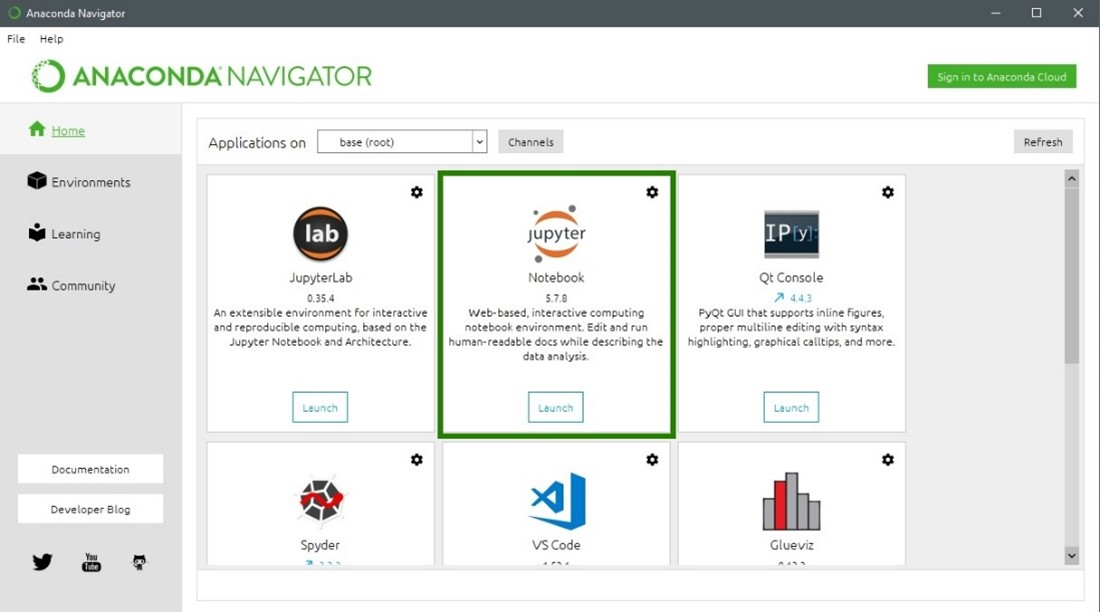
\includegraphics[width=1\textwidth]{images/anaconda.jpg}
\caption{\gls{anaconda} Navigator}
\label{fig:fig_01}
\end{figure}
\FloatBarrier

Theoretically, it would also have been possible for each developer to install \gls{anaconda} on their computer and work on the notebook, which is maintained on a Github repository. However, since the project is very hardware-heavy and compiling a machine learning model can take up to several hours, a \gls{virtual machine} turns out to be the better option.

\subsubsection{PyCharm}
is an integrated development environment (IDE) used for programming in the Python language, created by the Czech company JetBrains. I used it because it supports anaconda, git and as a debugger.
It natively supports jupyter notebooks is perfect because it is much more comfortable than jupyter itself, then it has several extensions that make programming easier and more intuitive.

\subsubsection{Github}
Provider with the function of hosting for software development and version control using Git.
Thanks to its free of charge nature it's used for most of the open-source projects.
That's why it's loved by the community of programmers, even I use it for this project to save files and use them from different locations.


\subsubsection{Overleaf}
Overleaf is cloud-based \LaTeX{} editor, which makes writing a scientific paper collaborative. \LaTeX{} is a software widely used in the academic world to create scientific texts, with useful formatting for mathematical, statistical, computer science, physics texts, which can be problematic on other text editors.
I preferred Overleaf to other solutions for the convenience, in fact there is no need to install anything, everything is accessible via the internet as with Colab.
Overleaf was useful for me to write this documentation, thanks also to its versioning nature.

\subsubsection{MLMP}
MLMP is a cloud-based environnement in which machine learning models can be trained. Similar to Colab, this environnement was created by the BFH Institute, to allow its students to be able to train models, with a more performing machine.It is possible to use it in the BFH network or through a connection to the network via VPN, the advantage lies in being able to use not only the CPU, as in normal virtual machines, but also very powerful GPUs, designed precisely for this purpose.This way I can train my model much faster, having much more computing power at my disposal.

These are the available environments:
\begin{figure}[ht!]
\centering
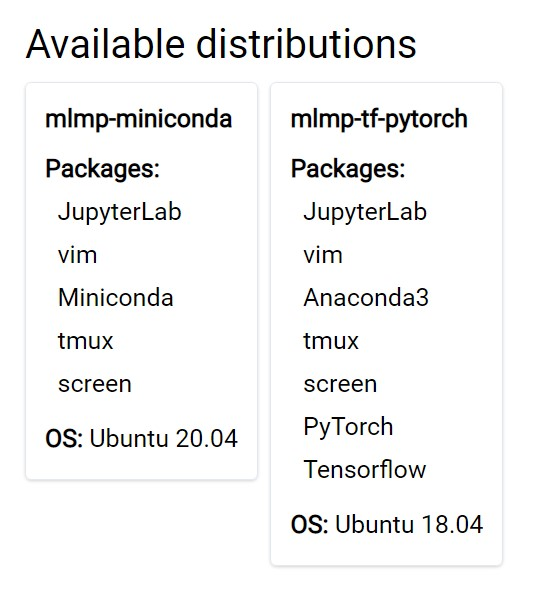
\includegraphics[width=0.5\textwidth]{images/bfhmlmp.jpg}
\caption{MLMP distributions}
\label{fig:fig_02}
\end{figure}
\FloatBarrier
Perchè ho scelto questo env?
differenze tra cpu e gpu, un paio di grafici e quale gpu ho usato
Un esempio di CPU vs GPU:

Come è possibile vedere la GPU ci mette molto meno tempo 

https://option40.com/blog/ml-how-much-faster-is-a-gpu


\subsubsection{Scikit-learn}
Scikit-learn is  a  free  software  machine  learning  library  for  the  Python  programming  lan-guage.It features various classification, regression and clustering algorithms includingsupport vector machines, random forests, gradient boosting, k-means and DBSCAN,and  is  designed  to  interoperate  with  the  Python  numerical  and  scientific  libraries NumPy and SciPy.

\subsubsection{Tensorflow}
Tensorflow is a machine learning framework from Google, which facilitates the process of capturing data, training models, making predictions, and refining future results.

TF is an open source library for large-scale numerical computing and machine learning, it bundles a number of machine learning and deep learning algorithms and models.
All this is provided through the python language; for the reason that it is easy to learn and implement.
The actual mathematical operations, however, are performed in high-performance c+.
\subsubsection{Keras}

\subsubsection{Ktrain}
ktrain is a lightweight wrapper for the deep learning library TensorFlow Keras (and other libraries) to help build, train, and deploy neural networks and other machine learning models. Inspired by ML framework extensions like fastai and ludwig, it is designed to make deep learning and AI more accessible and easier to apply for both newcomers and experienced practitioners.
ktrain provides support for applying many pre-trained deep learning architectures in the domain of Natural Language Processing and BERT is one of them. To solve this problem, we will be using the implementation of pre-trained BERT provided by ktrain and fine-tune it to classify whether the disaster tweets are real or not.

\subsubsection{BERT}
bert è stat of the art per fare le cose

BERT (Bidirectional Encoder Representations from Transformers) is a deep learning model developed by Google. Ever since it was open-sourced by Google, it has been adopted by many researchers and industries and has applied in solving many NLP tasks. The model has been able to achieve state of the art performance on most of the problems it has been applied upon.

9.	la difficoltà più grande è trovare la parte di bert che si addice meglio.
Infatti questo task ha bisogno di molto tempo e ricerca per poter capire quale bert faccia al caso mio.


\subsubsection{Hugging Face}
Transformers posso utilizzare perché mi da migliaia di modelli pre allenati per il taskt text classificazione, estrazione informazione, risposta a domande, ecc in più di 100 lingue.
NLP è diventato facile e accessibile per tutti.

